\documentclass{libtex/llncs}

\usepackage{url}
\usepackage{color}
\usepackage{paralist}
\usepackage{fancyvrb}
\usepackage{amsmath}
\usepackage{epsfig}
\usepackage{subfig}
\usepackage{float}
\usepackage[nomove]{cite}
\usepackage{tabularx}
\usepackage[table]{xcolor}
\usepackage{amssymb}
\usepackage{graphicx}
\usepackage{mdframed}
\usepackage{multirow}
%\usepackage[table,xcdraw]{xcolor}


\graphicspath{ {figures/} }


\newcommand{\new}[1]{{\color{blue}#1}}
\newcommand{\draft}[1]{{\color{red}#1}}
\long\def\comment#1{}
\newcommand{\q}[1]{\lq\lq{}{}#1\rq\rq{}{}}

\begin{document}

\title{
    Ranking Archived Documents for Structured Queries on Semantic Layers% and Time
    %Capturing Implicit User Search Preferences through Ranking Algorithms on Structured Data
}

\author{
    Vaibhav Kasturia \and
    Pavlos Fafalios \and
    Wolfgang Nejdl }

\institute{
    L3S Research Center, University of Hannover, Germany\\
    \email{\{kasturia, fafalios, nejdl\}@l3s.de} }



\maketitle


\begin{abstract}
Archived collections of documents (like newspaper and web archives)
serve as important information sources
in a variety disciplines, including Digital Humanities, Historical Science, and Journalism.
%for a variety of interested parties, such as historians, journalists and sociologists.
However, the absence of efficient and meaningful exploration methods
still remains a major hurdle in the way of turning them into usable sources of information.
Semantic Layers allow describing
and publishing metadata and semantic information about the archived documents in a standard format (RDF),
which in turn can be queried through a semantic query language (SPARQL).
This allows running advanced queries by combining
metadata of the documents (like publication date) and
content-based semantic information (like entities mentioned in the documents).
However, the results returned by structured queries
can be numerous and also they all equally match the query.
There is thus the need to rank the returned results in order to identify and promote the most important ones.
In this paper,
we formalize the problem of {\em ranking archived documents for structured queries},
we distinguish two main types of queries for this problem,
and we propose a baseline ranking model that jointly considers the following aspects:
i) the relativeness of documents to entities,
ii) the timeliness of documents, and
iii) the relations among the entities.
The results of an extensive experimental evaluation on a news archive are promising.
\end{abstract}



\section{Introduction}
%Digital archiving is the long-term electronic preservation and management
%of historical documents and assets in general.

Despite the increasing number of digital archives worldwide
(like newspaper and web archives), the absence of efficient and meaningful
exploration methods still remains the major bottleneck in the way of
turning them into usable information sources \cite{calhoun2014exploring}.
Semantic models try to solve this problem by offering the means
to describe metadata and semantic information
about a collection of archived documents in the standard RDF format.
A repository of such data, called Semantic Layer \cite{fafalios2017SemLayer},
allows running advanced queries which
combine metadata of the documents (like publication date) and
content-based semantic information (like entities mentioned in the documents).
As an example, we can access a Semantic Layer over a newspaper archive and
find articles of a specific time period discussing about a specific category of entities
(e.g., {\em philanthropists}) or about entities sharing some characteristics
(e.g., {\em lawyers born in Germany}).
Such advanced information needs can be directly expressed through structured (SPARQL) queries
or through user-friendly interactive interfaces
which transparently transform user interactions to SPARQL queries
(e.g., a faceted browsing interface \cite{tzitzikas2016faceted}).

However, the results returned by such queries can be numerous and
moreover they all equally match the query.
Thus, there arises the need for an effective method to rank the returned results
for discovering and promoting the most important ones.
As an example, when requesting articles from a news archive mentioning a specific entity,
some of the returned articles may be about that entity
while other articles may just mention the entity without it being their main topic.
Thus, an effective ranking method should
consider the different factors that affect the importance of documents to the information need,
relying at the same time only on the data
available in the semantic layer (without accessing documents' full contents).

Although there is a plethora of works on both
ranking archived documents for keyword-based queries
and ranking structured data (subjects and objects) in knowledge graphs,
the problem of ranking archived documents for structured queries in knowledge graphs
has not yet been recognized and studied.
In this paper, we address this gap by first introducing and formalizing this task
and then proposing a ranking model for the problem at hand.
The proposed model jointly considers the following aspects:
i) the {\em relativeness} of a document with respect to the entities of interest,
ii) the {\em timeliness} of document's publication date,
iii) the temporal {\em relatedness} of the entities of interest with other entities
mentioned in the document.
The idea is to promote documents that
mention the entities of interest many times,
that have been published in important (for the entities of interest) time periods, and that
mention many other entities co-occurring frequently
with the entities of interest in important time periods.
For example, in case we want to rank articles of 1990
discussing about {\em Nelson Mandela},
we want to favor articles that
i) mention {\em Nelson Mandela} multiple times in their text,
ii) have been published in important time periods for {\em Nelson Mandela}
(e.g., February 1990 since during that period he was released from prison), and
iii) mention other entities that seem to be important for {\em Nelson Mandela}
during important time periods
(e.g., {\em Frederik Willem de Klerk} who was
South Africa's State President in February 1990).

In a nutshell, in this paper we make the following contributions:
\begin{compactitem}
\item   We formulate and formalize the problem of ranking archived documents
        for structured queries over semantic layers.
\item   \draft{We proposed a ranking model for the problem at hand that ... ...}
\item   Due to lack of evaluation datasets for our problem, we have created
        a new ground truth dataset for a news archive which we make publicly available.
\item   \draft{The evaluation results show that the proposed ranking model ...}
\end{compactitem}
%For this problem, we should consider the different factors
%that affect the importance of a document to the information need,
%relying at the same time only on the data
%available in the semantic layer (without accessing documents' full contents).

\comment{====
    Archiving is the process of preservation of records
    permanently or for long-terms on grounds of their
    enduring cultural, evidentiary or historical value.
    As the web continues to grow we have records holding
    significant value being constantly produced
    and consumed every day. However, due to transient
    nature of the Web, most of these records produced
    become either lost or unavailable after a short period
    of time. Archives capture portions of these record
    collections for sociologists, historians and other interested
    parties for whom these collections are immensely valuable.

    Just as Archives contain historical records,
    in the same way Web Archives capture portions of the Web
    in order to preserve it for
    sociologists, historians, and other interested parties.
    For them, these collections form immensely valuable
    information sources for their work.
    These Web Archives contain snapshots of the Web sites
    at different points of time and are created by regularly
    crawling (parts of) the Web.

    With the number of archives increasing worldwide models,
    tools and techniques necessary to archive and index relevant
    parts of the web in order to create, retrieve and
    explore them in a meaningful way are being constantly suggested and developed.
    In our previous work\cite{fafalios2017SemLayer}, we proposed
    building semantic profiles/layers that describe information about
    the contents of the archived documents and could be used as a method to
    to solve the problem of archive exploration.
    Specifically, we used Semantic Web technologies as a base and
    constructed an RDF/S vocabulary that allowed for:
    a) describing useful metadata information about each archived
    document
    b) annotating each document with entities and events detected in its textual contents,
    c) enriching the detected entities/events\footnote{From now on,
        when we say \q{entities} we refer to both entities, events and concepts.} with more semantic information
    (like properties and related entities coming from the LOD), and
    d) publishing all this data on the Web in the standard RDF format
    (making thereby all this information directly accessible and exploitable by other systems and tools).
    The results showed that such semantic profiles/layers could meet complex information needs, especially {\em
    exploratory search} needs \cite{marchionini2006exploratory}.


    Even though {\em entity-centric} SPARQL queries on such structured data layers
    return relevant results, a shortcoming is sometimes the
    large number of results that we get for the
    queries that we submit. Moreover, all the
    results are equally relevant to the submitted query.
    This leads to the problem of the user judging which results he
    would want to consider to be \q{more} important than other results.
    For example, in the case of a user querying a {\em
    news archive} asking for \q{articles of 1988 asking about members of the German Parliament}, an implicit preference of
    the user would be to get those articles which might:
    a) have mentions of several members in the same article,
    b) have
    mentions of more prominent members to that time period rather than less prominent ones, and/or,
    c) contain members involved in significant events which happened during the time period.
    Thus, having algorithms to judge articles and return
    them in a ranked order would be useful for the user.


    To rank results, we propose ranking algorithms
    that take into account temporal aspects of entities, inter-relations
    between entities and relatedness of documents to entities.
    Our approach only exploits the data of the semantic repository
    (triples in RDF format) and thus
    can produce ranking at query-execution time.
    We based these algorithms by modelling the solutions of the
    following three problems:
    a) how to rank {\em documents} related to a time
    period and one or more entities,
    for example, articles mentioning former US President
    Barack Obama announcing a Nuclear Deal with Iran would be considered
    more important than him addressing the
    116th National Convention of the Veterans of Foreign Wars in Pittsburgh, PA,
    with both events having occurred in July 2015;
    b) how to rank {\em entities} related to a time period and one or more other
    entities, for example,
    Brexit is a more important entity related to former British Prime Minister David Cameron than American Intervention in Syria in 2016
    as he had to tender his resignation
    following the results of the Brexit polls;
    c) how to rank {\em time periods} related to one or more entities,
    for example, the period of September 2015 was a more
    significant period for the EU Chancellor Angela Merkel
    than July 2015 as the decision she made on letting trains filled with migrants enter Germany in during that time period led to a significant drop in her approval ratings\cite{merkel_rating}.


    We then evaluate whether our algorithms effectively solve these problems
    by running 20 {\em entity-centric} queries on a semantic layer of the {\em New York Times}
    archive and checking the result ranking against human relevance judgements to see which
    combination of the modelled factors leads to the best ranking.
====}

The rest of the paper is organized as follows:
Section \ref{sec:motivAndRW} motivates our work and presents related literature.
Section \ref{sec:queryingSemLayer} presents \new{basic} algorithms for ranking documents, entities, and time periods.
\new{Section \ref{sec:pagerank} tries to describe a probabilistic approach for the problem at hand.}
Section \ref{sec:eval} evaluates the algorithms and their combinations.
Finally, Section \ref{sec:concl} concludes the paper and
presents interesting directions for future research.




%=====================================================

\section{Background and Related Works (DRAFT)}
\label{sec:motivAndRW}




In this section, we first provide a background of the
{\em Open Web Archive} Data Model in which we describe the data model
along with a sample depiction of a non-versioned article as
in the semantic layer.
Then we mention the different works related to ranking of archived documents,
ranking in knowledge graphs and
ranking documents in knowledge graphs.

\subsection{The \q{Open Web Archive} Data Model}
\label{subsec:semanticmodel}

\-\hspace{0.5cm}In our previous work\cite{fafalios2017SemLayer} we introduced an RDF/S data model to describe
the semantic information and metadata about the documents
of a web archive.
This model, which we call as {\em Open Web Archive} data model\footnote{Specification publicly
available at: \url{http://l3s.de/owa/}},
is depicted in Figure \ref{fig:owa}.
We re-use elements from many other existing data models
and define 2 new classes and 3 new properties.
An archived document is represented using the class {\tt owa:Archi\-ved\-Do\-cu\-ment}.
Further, the archived document may or may not be linked with some versions
(i.e., instances of {\tt owa:Ve\-rsio\-ned\-Do\-cu\-ment}).
Versions pages for billions of web sites can be
found on the Internet Archive.
In contrast, the New York Times corpus \cite{sandhaus2008new} that we
try applying our ranking models on does
not contain versions.

We associate an archived document
with three main elements:
i) metadata information, like format(mime type),
date of capture/publication, and document title,
ii) links to other documents (web pages), archived or not, and
iii) set of annotations.
Terms from the Dublin Core Metadata Initiative\footnote{\url{http://dublincore.org/}}
were used to describe some of the metadata.
Annotations were described by exploiting
the Open Annotation Data Model \cite{sanderson2013open}
and the Open Named Entity Extraction (NEE) Model \cite{fafalios2015ijait}. % \footnote{\url{http://www.ics.forth.gr/isl/oae/}}

The Open Annotation Data Model contains an RDF-based framework specification for creating associations (annotations)
between related resources, while the Open NEE Model is an extension
that allows describing the result of an entity extraction process.
An annotation has a {\em target}, which is an archived document in our case, and
a {\em body} which is a concept, entity or event
mentioned in the document.
An archived document can be directly related with an
entity, concept or event by exploiting the property \q{{\tt mentions}}
of schema.org\footnote{\url{http://schema.org/mentions}} for reducing the
number of derived triples.
A concept, entity or event can be associated with information like
its name, a confidence score, its position in the document, and a resource (URI).
The URI enables to retrieve additional information from the Linked Open Data (LOD)
cloud \cite{heath2011linked} (like properties, relations with other entities, etc.).

\begin{figure}[H]
\centering
\fbox{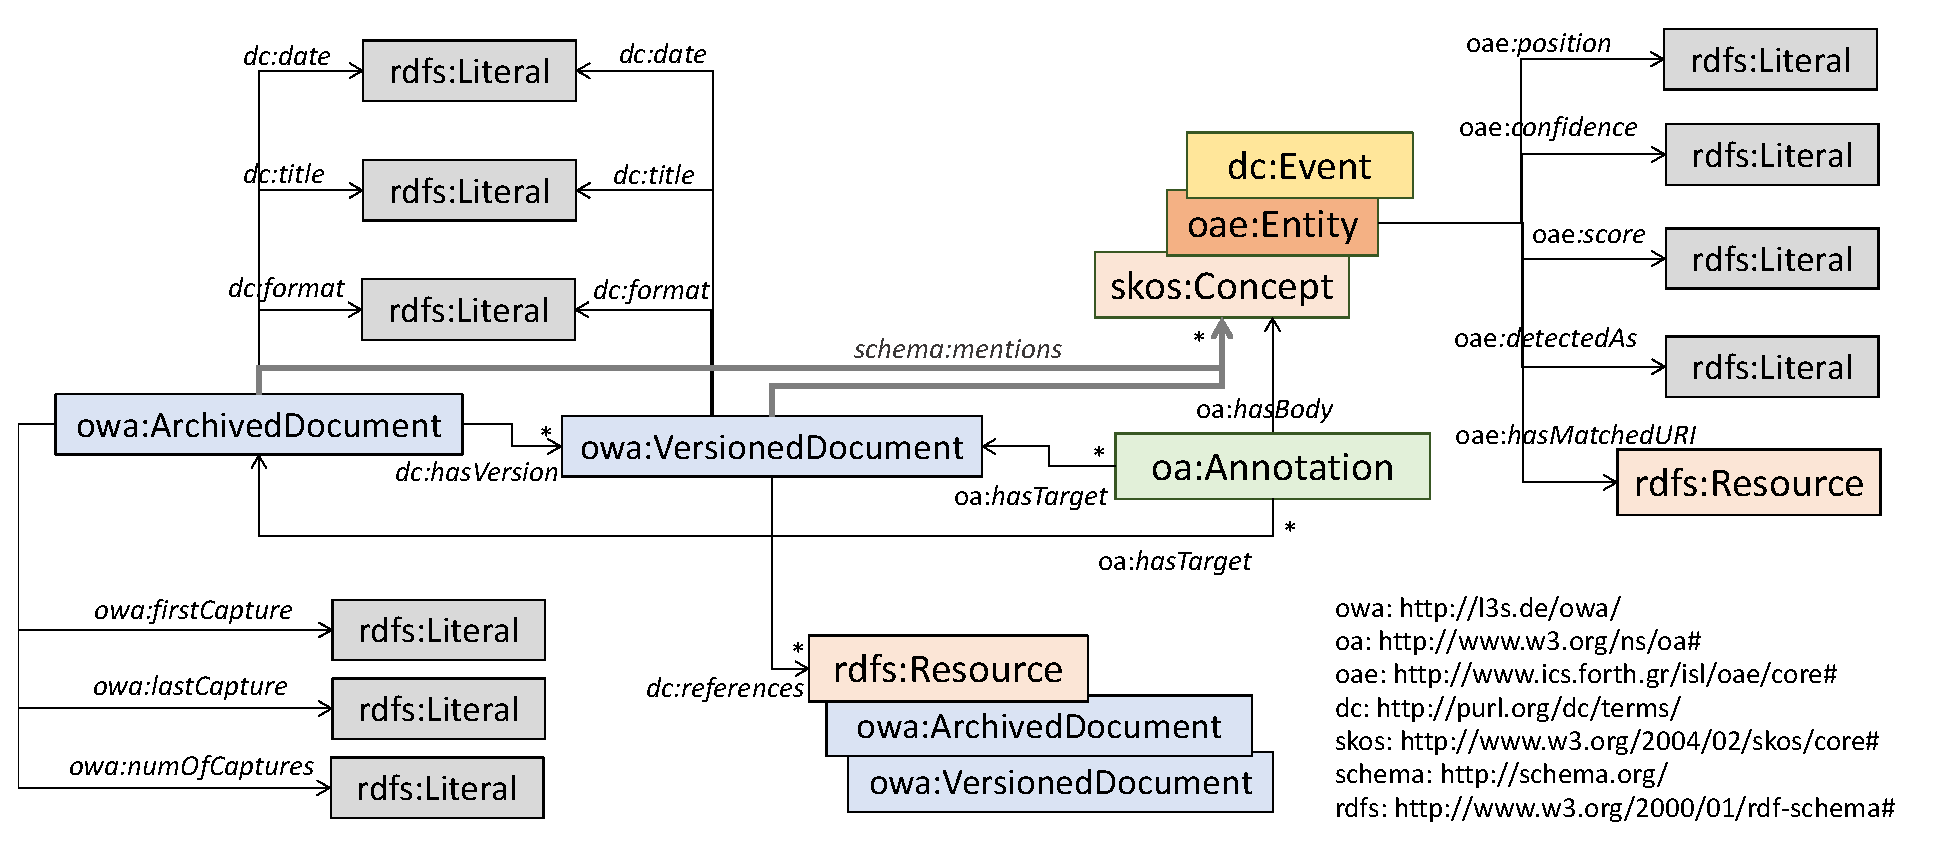
\includegraphics[width=\dimexpr\textwidth-2\fboxsep-2\fboxrule\relax]{figures/owa.eps}}
\caption{The {\em Open Web Archive} data model.}
\label{fig:owa}
\end{figure}

\begin{figure}[H]
\centering
\fbox{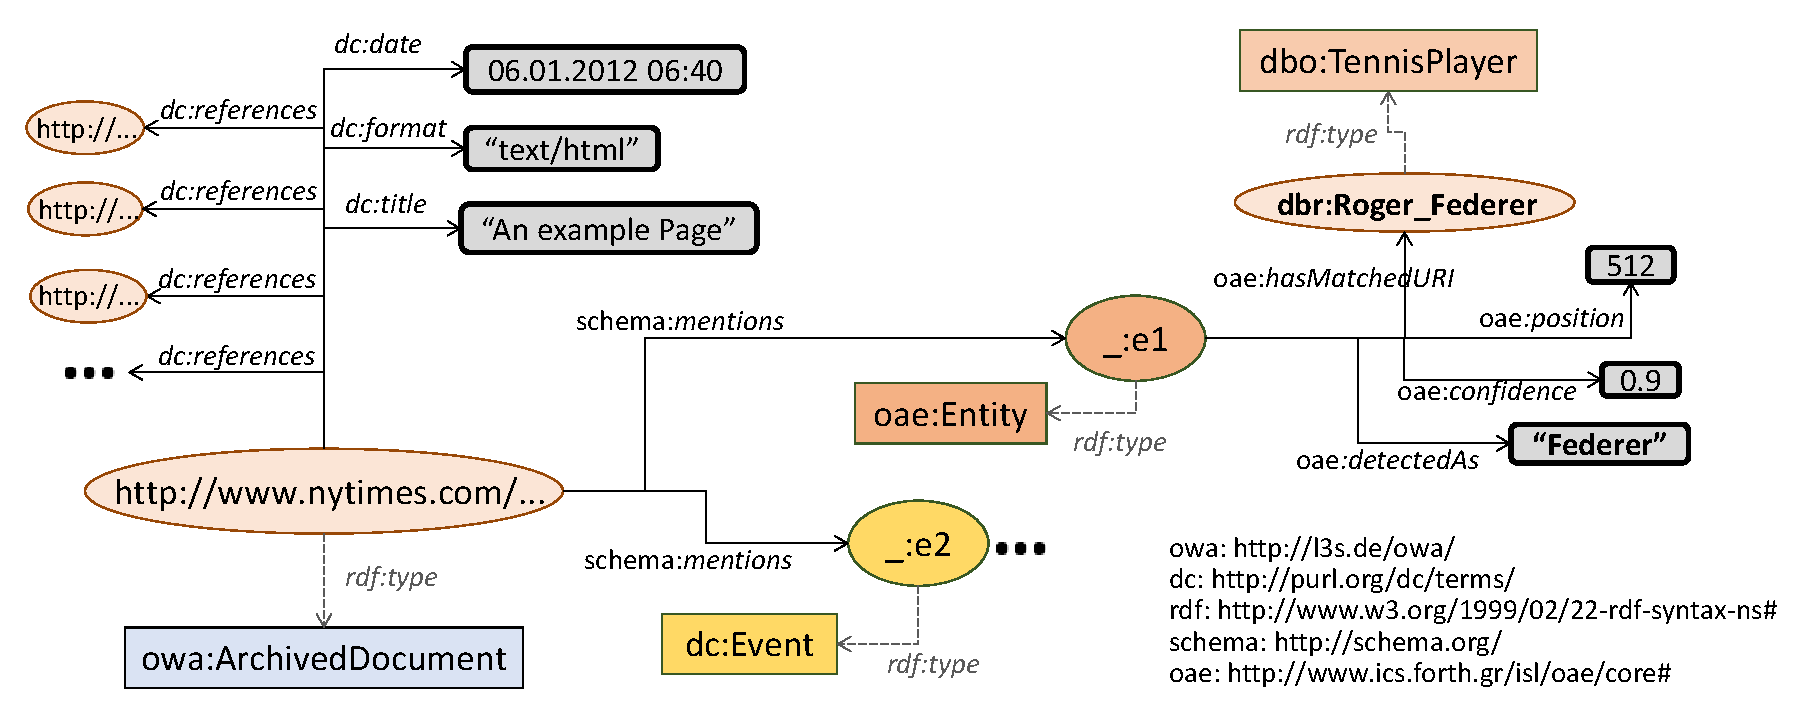
\includegraphics[width=\dimexpr\textwidth-2\fboxsep-2\fboxrule\relax]{figures/owa_inst_nonvers.eps}}
\caption{Describing an archived article (non-versioned) using the {\em Open Web Archive} data model.}
\label{fig:owa_instNonVers}
\end{figure}

Figure \ref{fig:owa_instNonVers} depicts an example of an archived non-versioned article.
Some of its metadata values (date, format, title),
its references to other web pages, and its annotations are visible.
We notice that the entity name \q{Federer} was identified
in that document.
It is also visible that the entity has been linked with the DBpedia resource
corresponding to the tennis player {\em Roger Federer}.
By accessing DBpedia, we can now retrieve more information about this entity
like its birth date, an image, a description in a specific language, etc.
Description of versioned pages using {\em Open Web Archive}
data model is not mentioned in this paper since our
work is mainly focussed on ranking on non-versioned pages.
Details of the construction process of Semantic Layers
have also not been included.
Interested readers should refer to our previous work\cite{fafalios2017SemLayer}
for a more detailed description of this model.

\comment{====
\vspace{0.5mm} \noindent
{\bf Extensibility and Update.}
The proposed model is highly extensible.
For instance, we can
exploit the VoID Vocabulary \cite{alexander2011describing}
and express dataset-related information like
statistics (number of triples, number of entities, etc.),
creation or last modification date,
the subject of the dataset,
collection from which the dataset was derived, etc.
Likewise, one may exploit the PROV data model \cite{moreau2013prov}
and store provenance-related information
(e.g., which tool was used for crawling the documents or for annotating them,
what organizations or people were involved in the crawling or annotation process,
etc.).
In addition, since the contents of the archived documents never change,
we can easily update a semantic layer by just
adding triples in the RDF repository,
e.g., for describing more metadata about the archived documents
or for including new versions.
=====}

\subsection{Related Work (DRAFT)}
\label{rw}

\subsubsection{Ranking of Archived Documents}
\label{arc_doc_ranking}
We mention some of the recent works in the
field of ranking of Archived Documents
using full content based search
or extraction of metadata.

Tempas \cite{holzmann2016tempas}
is a keyword-based search system that exploits a social bookmarking service for
temporally searching a web archive by indexing tags and time.
It allows temporal selections
for search terms, ranks documents based on their
popularity and also provides query recommendations.

Singh et al.\cite{singh2016history}
introduce the notion of {\em Historical Query Intents}
and model it as a search result diversification task
which intends to present the most relevant results (for free text queries) from a
topic-temporal space.
For retrieving and ranking historical documents (e.g., news articles),
the authors propose a novel retrieval algorithm, called HistDiv,
which jointly considers the aspect and time dimensions.

Expedition \cite{singh2016expedition} is a time-aware
search system for scholars.
It allows users to search articles in a news
collection by entering free-text queries and choosing
from four retrieval models:
Temporal Relevance,
Temporal Diversity,
Topical Diversity, and
Historical Diversity.
\comment{====
The results are presented in a
newspaper-style interface, while entity filters
allows users refine the results.
====}

\comment{=====
Excluded as Sindice deals with
RDF Documents in general and
not archived documents.

Sindice\cite{tummarello2007sindice} acts as a locator
service for RDF resources and
returns pointers to the remote data sources.
The ranking is metadata based and
the service ranks the results obtained
after index retrieval on query time
based upon a resource's hostname, external rank
and relevance.
====}

\noindent \textbf{Difference of our approach.} Our approach
provides ranking using structured queries rather than
keyword-based queries.
To provide ranking, we do not access
the content of the articles rather a
layer composed of RDF triples which
contains metadata, links and entities
extracted from the articles.

\subsubsection*{Ranking in Knowledge Graphs}
\label{graph_ranking}

Most of the Ranking Approaches on Knowledge Graphs
are adaptations
of the existing approaches for unstructured data.

Dali et. al.\cite{dali2012query} propose a query
independent Learning to Rank(LTR) approach
for RDF entity search. They use RDF graph extracted features,
search engine based features
and centrality-based features and compare them to target features.
Latifi and Nematbaksh\cite{latifi2014query} also use
the same approach
but suggest the use of Information Content(IC) feature
to reduce ranking time of the system.

OntologyRank algorithm by Ding et al. introduced
in \cite{ding2004swoogle} and mentioned
further in \cite{ding2005finding}
finds use in the Semantic web search engine \emph{Swoogle}.
It identifies Semantic Web Ontologies(SWOs) in Semantic Web
Documents(SWDs) and further ranks terms in an Ontology based on their popularity.
AKTiveRank\cite{alani2006ranking} by Alani et. al.
is another ontology ranking approach which relies
on their importance to a given query
and uses the semantic web search engine
\emph{Swoogle}\cite{ding2005finding} to get a list
of ontologies that need to be ranked.
SemRank\cite{anyanwu2005semrank} designed by
Anwanyu et. al. ranks relationships in SWDs.

Regarding PageRank based approaches, PopRank\cite{nie2005object} 
assigns weights to links among Web Objects
depending on the relationship types between objects.
This system extracts a subset of the graph
based on domain and then assigns link weights
to the subgraph using expert generated Ranking Lists.
Harth et. al.\cite{harth2009using} perform ranking 
by assigning weights to all links in the graphs
based on authority or provenance of data source
and calculating PageRank for the whole
graph even before the query is entered.
This approach is in complete contrast
to ReConRank\cite{hogan2006reconrank}, an
algorithm that performs dynamic ranking only
analysing the result data that matches the user query and 
which considers the ratio of all the links received as
in-links in order to reduce the number of iterations.
RareRank\cite{wei2009semantic} is another 
algorithm where the random component
in the PageRank model is replaced by
a more deterministic component based on
the domain of search in order to reduce randomness in a graph.
DBPediaRanker\cite{mirizzi2010ranking} 
first dereferences and explores all nodes in the
DBPedia graph belonging to the same
domain given a query. Then by checking whether
a strong relation exists between two resources,
it creates a contextualized weighted graph.
YAGO-NAGA introduced in Kasneci et. al.\cite{kasneci2008naga}
and extended to include keyword based search in
Elbassouni et. al.\cite{elbassuoni2009language} is
a semantic search system based on Language Model that
performs ranking based on the notions of Informativeness,
Compactness and Confidence.
DING\cite{delbru2010hierarchical} 
calculates rank in three steps:
first the global dataset rank,
then the entity rank and finally the global ranking
which is a combination of the of both the global
dataset rank and the entity rank.
Fafalios and Tzitzikas\cite{fafalios2014post} integrate
classical Web with the LOD Web using PageRank like algorithm 
to provide users with semantic context 
to help them save
time in exploratory search scenarios.
 
Considering link-based approaches other than
PageRank adaptations, 
NOC-ORDER\cite{graves2008method} introduced by
Graves et. al. is an adaptation of \emph{All-Pairs Shortest Path}
algorithm that ranks nodes in an RDF graph
based on centrality feature.

\comment{====
Older Version(use in case more space available and 
approaches need to be described in greater detail.)

Dali et. al.\cite{dali2012query} propose a query
independent Learning to Rank(LTR) approach
for RDF entity search. They use RDF graph extracted features,
search engine based features
and centrality-based features and compare them to target features.
To obtain the ground truth for the target
features they use human relevance judgements.

Latifi and Nematbaksh\cite{latifi2014query} use
the same approach as that proposed
by Dali et. al.\cite{dali2012query}
but suggest the use of the Information Content(IC) feature
to reduce ranking time of the system.

SemRank\cite{anyanwu2005semrank} designed by
Anwanyu et. al. ranks relationships instead of entities.
The final ranking is calculated based on the predictability
or gain of information of
a semantic association, the degree of similarity
of a keyword or property occurring in a semantic association
and the amount of differences between the properties
in the original schema and the properties that compose a path.

OntologyRank algorithm by Ding et al. introduced
in \cite{ding2004swoogle} and mentioned
further in \cite{ding2005finding}
finds use in the Semantic web search engine \emph{Swoogle}.
It identifies Semantic Web Ontologies(SWOs) in Semantic Web
Documents(SWDs) and further ranks terms in an Ontology based on their popularity.

PopRank\cite{nie2005object} is a variation of PageRank
that assigns weights to links among Web Objects
depending on the relationship types between objects.
This system extracts a subset of the graph
based on domain and then assigns link weights
to the subgraph using Ranking Lists made by domain experts.

ReConRank\cite{hogan2006reconrank} is a PageRank
based algorithm that performs dynamic ranking and only
analyses the result data that matches the user query.
It considers the ratio of all the links received as
in-links in order to reduce the number of iterations
and allows users to fine tune the weights according to their choice.
It goodness relies on the relationships between resources
and their provenance and faces challenges
like extraction of topical graph and increase
in query time due to dynamic ranking.

AKTiveRank\cite{alani2006ranking} by Alani et. al.
is another ontology ranking approach which relies
on their importance to a given query
and uses the semantic web search engine
\emph{Swoogle}\cite{ding2005finding} to get a list
of ontologies that need to be ranked.

YAGO-NAGA introduced in Kasneci et. al.\cite{kasneci2008naga}
and extended to include keyword based search in
Elbassouni et. al.\cite{elbassuoni2009language} is
a semantic search system based on Language Model that
performs ranking based on the notions of Informativeness,
Compactness and Confidence.
The computation is done through a PageRank
like algorithm and
makes use of the provenance of information.

Harth et. al.\cite{harth2009using} use a variation
of the PageRank algorithm for ranking in which
they assign weights to all links in the graphs
based on authority or provenance of data source
and calculate PageRank for the whole
graph even before the query is entered.
This approach is in complete contrast
to ReConRank\cite{hogan2006reconrank} approach.

RareRank\cite{wei2009semantic} is another PageRank
like algorithm where the random component
in the PageRank model is replaced by
a more deterministic component based on
the domain of search in order to reduce randomness in a graph.

DBPediaRanker\cite{mirizzi2010ranking} tries to
first dereference and explore all nodes in the
DBPedia graph belonging to the same
domain given a query. Then by checking whether
a strong relation exists between two resources,
it creates a contextualized weighted graph
with the weights of links between two resources
based on the similarity between nodes.

DING\cite{delbru2010hierarchical} is another adaptation
of the PageRank algorithm which calculates rank in three steps.
First it calculates the global dataset rank,
then the entity rank and finally the global ranking
which is a combination of the of both the global
dataset rank and the entity rank.

NOC-ORDER\cite{graves2008method} introduced by
Graves et. al. ranks nodes in an RDF graph
based on centrality feature.
The algorithm is an adaptation of \emph{All-Pairs Shortest Path}
algorithm for RDF graph and tries to
rank nodes based on the connectedness
and distance of each node to the other nodes.

Fafalios and Tzitzikas\cite{fafalios2014post} integrate
classical Web with the Web of Linked Data to provide
users with semantic context and thus help users save
time in exploratory search scenarios.
For the top-100 results from BING search engine
for keyword search query, the system detects the entities in the snippets of the
results. For the top-k entities derived from a PageRank like algorithm,
the system then using the information available
on the LOD Cloud tries
to show the user how the top detected entities are related.

====}

\noindent \textbf{Difference of our approach.} Our work ranks documents
rather than entities, relationships \cite{anyanwu2005semrank}
or ontologies (\cite{ding2004swoogle}, \cite{ding2005finding}
and \cite{alani2006ranking}).
Unlike \cite{dali2012query} and
\cite{latifi2014query}, our approach does not require any training data.
It does not use any kind of link analysis like in \cite{hogan2006reconrank}, \cite{kasneci2008naga},
\cite{elbassuoni2009language}, \cite{harth2009using}, \cite{wei2009semantic}, \cite{delbru2010hierarchical}
and \cite{graves2008method}.
Further, its not domain specific like \cite{anyanwu2005semrank} and \cite{nie2005object},
doesn't rely on provenance of data sources as in \cite{kasneci2008naga}, \cite{elbassuoni2009language} and \cite{harth2009using} and
produces the ranking at query-execution time unlike \cite{hogan2006reconrank}.

\subsubsection{Ranking Documents in Knowledge Graphs}
\label{sec:graph_doc_ranking}
Little work has been done on ranking documents
in knowledge graphs.

Swoogle, the Semantic web search engine, uses
the OntologyRank algorithm \cite{ding2004swoogle}, \cite{ding2005finding}
as mentioned in the previous sub-section and operates at the document level
as well as the term and RDF graph level. It calculates relevance
of Semantic Web Documents based on whether a document imports,
uses, extends definition of the other document's terms or
makes assertions about the individuals defined by the other document.

\noindent \textbf{Difference of our approach.} Our approach does
not judge relevance of documents based on the relationships
between the documents, because our problem
is to rank a set of relevant documents rather than rank on the relevance
of documents. To the best of our knowledge, we are the very first authors
to perform such ranking using Semantic Models/Layers.

%=====================================================

\section{Ranking Documents for Structured Queries}
\label{sec:queryingSemLayer}


In this section, we formalize the problem of ranking documents returned by
structured (SPARQL) queries and define a probabilistic ranking model.
First we introduce the required notions and notations.

\subsection{Notions and Notations}

\subsubsection{Entities.}
In our problem, an {\em entity} is anything with a separate and meaningful existence
that also has an identity expressed through a reference in a knowledge base (e.g., a Wikipedia/DBpedia URI).
This does not only include persons, locations, organizations, etc., but also
events (e.g., {\em US 2016 presidential election})
and more abstract concepts such as {\em democracy} or {\em apartheid}.
Let $E$ be a finite set of entities, e.g., all Wikipedia entities,
where each entity $e \in E$ is associated with a unique URI in the reference knowledge base.

\comment{====
    \vspace{2mm} \noindent
    {\bf Documents and extracted entities}.
    Let $D$ be a set of documents, e.g., a set of news articles.
    For a document $d \in D$, let $publ(d)$ denote its publication date.
    Let also  $ents(d) \subseteq E$ be all entities mentioned in $d$.
    %(actually the URIs of these entities\footnote{From now on, when we say \q{entity} we mean \q{web entity URI}.}).
    Inversely, for an entity $e \in E$, let $docs(e) \subseteq D$
    be all documents that mention $e$, i.e., $docs(e) = \{d \in D ~|~ e \in ents(d)\}$.
    For an entity $e \in E$ and a document $d \in D$,
    let $count(e, d)$ be the number of occurrences of $e$ in $d$.
    %Now, let $ef(e, d) = \frac{count(e, d)}{\sum_{e' \in ents(d)}{count(e', d)}}$ be the
    %(normalized) frequency of $e$ in $d$.
    Finally, let $E_D$ be all entities mentioned in documents of $D$,
    i.e., $E_D = \cup_{d \in D}{ents(d)}$.

    \vspace{2mm} \noindent
    {\bf Time periods}.
    Let $\Delta$ be a fixed time period granularity (e.g., {\em day}).
    Based on a granularity $\Delta$,
    let $T = (t_0, t_1, \dots, t_n)$ be an ordered list of consecutive time points
    covering the publication dates of all documents in $D$.
    Note that $t_i - t_{i-1} = \Delta$, for each $i \geq 1$.
    Now, let $\delta_i = [t_i, t_{i+1})$ be the time period of size $\Delta$ between two consecutive time points.
    We consider that a document $d$ is published in the period $\delta_i$, if $t_i \leq publ(d) < t_{i+1}$.
    For a document $d \in D$, let $p_d$ be the time period in which $d$ was published.
    Now, let $P_D$ denote the set of distinct time periods of all documents in $D$,
    i.e., $P_D = \cup_{d \in D}{\{p_d\}}$.
    For a time period $p \in P_D$, let $docs(p) \subseteq D$ be the set of all
    documents published within $p$, i.e., $docs(p) = \{d \in D ~|~ p_d = p\}$,
    and $ents(p) \subseteq E_D$ be the set of
    entities discussed in documents of $D$ published within $p$,
    i.e., $ents(p) = \cup_{d \in docs(p)}{ents(d)}$.
====}

\subsubsection{Documents and extracted entities.}
Let $D$ be a set of documents (e.g., a set of news articles)
published within a set of time periods $T_D$ of fixed granularity $\Delta$ (e.g., day).
For a document $d \in D$, let $t_d \in T_D$ be the time period of granularity $\Delta$ in which $d$ was published,
while for a time period $t \in T_D$, let $docs(t) \subseteq D$ be the set of all
documents published within $t$, i.e., $docs(t) = \{d \in D ~|~ t_d = t\}$.

Let now  $ents(d) \subseteq E$ be all entities mentioned in $d$.
Inversely, for an entity $e \in E$, let $docs(e) \subseteq D$
be all documents that mention $e$, i.e., $docs(e) = \{d \in D ~|~ e \in ents(d)\}$.


%and $ents(p) \subseteq E_D$ be the set of
%entities discussed in documents of $D$ published within $p$
%(i.e., $ents(p) = \cup_{d \in docs(p)}{ents(d)}$).


\subsection{Problem Definition}
Given a corpus of documents $D$,
a set of entities $E_D$ mentioned in documents of $D$,
and a SPARQL query $Q$ requesting documents from $D$
published within a {\em time period} $T_Q \subseteq T_D$ and
related to one or more query entities $E_Q \subseteq E_D$
with logical {\tt AND} (mentioning all the query entities) or {\tt OR} (mentioning at least one of the query entities) semantics,
the problem is how to rank the documents $D_Q \subseteq D$ that (equally) match $Q$.

Figure \ref{fig:modelingExampleQ1} shows an example SPARQL query
requesting documents published in 1990
discussing about the entities {\em Nelson Mandela} %(\url{http://dbpedia.org/resource/Nelson_Mandela})
and {\em Frederik Willem de Klerk} %(\url{http://dbpedia.org/resource/F._W._de_Klerk}).
({\tt AND} semantics),
while the query in Figure \ref{fig:modelingExampleQ2} requests
articles of 1990 discussing about {\em state presidents of South Africa}
({\tt OR} semantics).
Our objective is to rank the results returned by such SPARQL queries.


\begin{figure}[th]
\vspace{-4mm}
\centering \scriptsize
\begin{Verbatim}[frame=lines,numbers=left,numbersep=1pt]
SELECT DISTINCT ?article WHERE {
  ?article dc:date ?date FILTER(?date >= "1990-01-01"^^xsd:date &&
                                ?date <= "1990-12-31"^^xsd:date) .
  ?article oae:mentions ?entity1, ?entity2 .
  ?entity1 oae:hasMatchedURI  <http://dbpedia.org/resource/Nelson_Mandela> .
  ?entity2 oae:hasMatchedURI  <http://dbpedia.org/resource/F._W._de_Klerk> }
\end{Verbatim}
\vspace{-5.5mm}
\caption{SPARQL query for retrieving articles of 1990 discussing
about {\em Nelson Mandela} and {\em Frederik Willem de Klerk} ({\tt AND} semantics).}
\label{fig:modelingExampleQ1}

%\vspace{-4mm}
\centering \scriptsize
\begin{Verbatim}[frame=lines,numbers=left,numbersep=1pt]
SELECT DISTINCT ?article WHERE {
  SERVICE <http://dbpedia.org/sparql> {
    ?p dc:subject <http://dbpedia.org/resource/Category:State_Presidents_of_South_Africa> }
  ?article dc:date ?date FILTER(?date >= "1990-01-01"^^xsd:date &&
                                ?date <= "1990-12-31"^^xsd:date)
  ?article oae:mentions ?entity .
  ?entity oae:hasMatchedURI  ?p }
\end{Verbatim}
\vspace{-5.5mm}
\caption{SPARQL query for retrieving articles of 1990 discussing
about {\em state presidents of South Africa} ({\tt OR} semantics).}
\label{fig:modelingExampleQ2}
\vspace{-4mm}
\end{figure}



\subsection{Probabilistic Modeling}

We model and estimate the probability to select a document $d \in D_Q$
given the query entities $E_Q$, the time period of interest $T_Q$,
and other entities $E_{D_Q}$ mentioned in the retrieved documents.
Specifically, we model the following aspects:
\begin{itemize}
\item the {\em relativeness} of a document with respect to the query entities
\item the {\em timeliness} of a document with respect to its publication date
\item the {\em relatedness} of a document with respect to its reference to other entities related to the query entities
\end{itemize}
% iv) the {\em temporal closeness} of a document with respect to other documents.}
The idea is to promote documents that
mention the query entities many times in their contents,
have been published in important (for the query entities) time periods, and
mention many other entities that co-occur frequently with the query entities in important time periods.
For example, in case we want to rank articles of 1990
discussing about {\em Nelson Mandela},
we want to favor articles that
i) mention {\em Nelson Mandela} multiple times in their text,
ii) have been published in important (for {\em Nelson Mandela}) time periods
(e.g., February of 1990 since during that period he was released from prison), and
iii) mention other entities that seem to be important for Nelson Mandela
during important time periods
(e.g., {\em Frederik Willem de Klerk} who was
South Africa's State President in 1990).

\subsection*{Relativeness}

We consider that if the query entities are mentioned multiple times
within a document, the document should receive a high score
(since the document's topic may be about these entities).
The term frequency (in our case entity frequency) is a classic numerical statistic
that is intended to reflect how important
a word is to a document in a collection or corpus \cite{leskovec2014mining}.

We first define a {\em relativeness} score of a document $d \in D_Q$
based on the {\em frequency} of the query entities in $d$.
First, let $count(e, d)$ be the number of occurrences of $e$ in document $d$.
For the case of {\tt AND} semantics (\q{$\wedge$}),
the score is defined as follows:
\begin{equation}
\small
score^{f}_{\wedge}(d, E_Q) = \frac{\sum_{e \in E_Q}{count(e, d)}}{\sum_{e' \in ents(d)}{count(e', d)}}
\end{equation}
Notice that the score of a document will be $1$ if it contains the query entities and no other entity.
For the case of {\tt OR} semantics (\q{$\vee$}),
we can also consider the number of query entities mentioned in the document
(since a document does not probably contain all the query entities as in the case of {\tt AND} semantics).
In that case, the {\em relativeness} score can be defined as follows:
\begin{equation}
\small
score^{f}_{\vee}(d, E_Q) = \frac{\sum_{e \in E_Q}{count(e, d)}}{\sum_{e' \in ents(d)}{count(e', d)}} \cdot \frac{|ents(d) \cap E_Q|}{|E_Q|}
\end{equation}
where $\frac{|ents(d) \cap E_Q|}{|E_Q|}$ is the percentage of query entities discussed in the document.
The score of a document will be 1 if it contains all the query entities and no other entity.
This formula favors documents mentioning multiple times many of the query entities.

Now, the probability of a retrieved document $d \in D_Q$ given only the query entities can be defined as:
\begin{equation}
\small
P(d|E_Q) = \frac{score^{f}(d, E_Q)}{\sum_{d' \in D_Q}{score^{f}(d', E_Q)}}
\end{equation}
%Notice that the above formula is a probability distribution of all returned documents.


\subsection*{Timeliness}

We consider that a time period $t \in T_Q$ is important
for the entities in $E_Q$, if there is a relatively big number of documents in $D_Q$
discussing about these entities during $t$.
For example, a big number of articles about {\em Nelson Mandela}
was published the period 11-13 of February 1990 because
in February 11 {\em Nelson Mandela} was released from prison.
Thus, articles published during that period should be promoted since
they are probably related to this important event of {\em Nelson Mandela}'s life.

For the case of {\tt AND} semantics,
we define the following importance score of a {\em time period} $t \in T_Q$:
\begin{equation}
score^{t}_\wedge(t) = \frac{|docs(t) \cap D_Q|}{|D_Q|}
\end{equation}
This scoring formula favors time periods in which there is a big number
of documents discussing about the query entities.

For the case of {\tt OR} semantics,
in a time period $t$ there may be a
big number of documents discussing only for one of the query entities,
while in another time period $t'$ there may be a smaller number
of documents discussing though for many of the query entities.
For also taking into account the number of query entities discussed in documents
of a specific time period, we consider the following formula:
\begin{equation}
\small
score^{t}_\vee(t) = \frac{|docs(t) \cap D_Q|}{|D_Q|} \cdot N(E_Q,t)
\end{equation}
where, $N(E_Q,t)$ is the average percentage of query entities discussed in articles of $t$, i.e.:
\begin{equation}
\small
N(E_Q,t) =  \frac{\sum_{d \in docs(t) \cap D_Q}{\frac{|ents(d) \cap E_Q|}{|E_Q|}}}{|docs(t) \cap D_Q|}
\end{equation}

Now, the probability of a retrieved document $d \in D_Q$ given only its publication date $t_d$ can be defined as:

\begin{equation}
\small
P(d | t_d) = \frac{score^{t}(t_d)}{\sum_{d' \in D_Q}{score^{t}(t_{d'})}}
\end{equation}



\subsection*{Relatedness}

Entities that are co-mentioned frequently with the query entities
in important time periods are probably important.
For example, {\em Apartheid} was an important concept
related to {\em Nelson Mandela} %and {\em Frederik Willem de Klerk}
during 1990,
thus articles discussing for both {\em Apartheid} and {\em Nelson Mandela} %, and {\em Frederik Willem de Klerk}
should be promoted.
However, there may be also some general entities (e.g., {\em South Africa} in our example)
that co-occur with the query entities in almost all documents (independently of the time period).
Thus, we should also avoid over-emphasizing documents mentioning such \q{common} entities.
%(in a similar way to the computation of {\em tf-idf} in IR).

For the case of {\tt AND} semantics,
we consider the following {\em relatedness} score
for an entity $e \in E_D \setminus E_Q$:

\begin{equation}
\begin{split}
\small
score^{r}_\wedge(e) = & ~ idf_\wedge(e) \cdot \sum_{t \in T_Q}{(score^{t}_\wedge(t) \cdot \frac{|docs(t) \cap D_Q \cap docs(e)|}{|docs(t) \cap D_Q|})}\\
= & ~ idf_\wedge(e) \cdot \sum_{t \in T_Q}{\frac{|docs(t) \cap D_Q \cap docs(e)|}{|D_Q|}}
\end{split}
\end{equation}
where $idf_\wedge(e)$ is the inverse document frequency
of entity $e$ in the set of documents discussing about the query entities in the entire corpus,
which can be defined as follows:
\begin{equation}
\label{frml:idf_and}
\small
idf_\wedge(e) = 1 - \frac{|docs(e) \cap (\cap_{e' \in E_Q}{docs(e')})|}{|\cap_{e' \in E_Q}{docs(e')}|}
\end{equation}
The formula considers the percentage of
documents in which the entity
co-occurs with the query entities in important time periods.

For the case of {\tt OR} semantics,
the above formula does not consider the
number of different query entities discussed in documents together with the entity $e$.
To also handle this aspect,
we consider the following {\em relatedness} score for the case of {\tt OR} semantics:
\begin{equation}
\begin{split}
\small
score^{r}_\vee(e) =  & ~ idf_\vee(e) \cdot  N(E_Q, e) \cdot \sum_{t \in T_Q}{(score^{t}_\vee(t) \cdot \frac{|docs(t) \cap D_Q \cap docs(e)|}{|docs(t) \cap D_Q|})} \\
= & ~ idf_\vee(e) \cdot N(E_Q, e) \cdot  \sum_{t \in T_Q}{(N(E_Q, t)\cdot \frac{|docs(t) \cap D_Q \cap docs(e)|}{|D_Q|})}
\end{split}
\end{equation}
where $N(E_Q, e)$ is
the average percentage of query entities discussed in articles together with entity $e$, i.e.:
\begin{equation}
\small
N(E_Q, e) =  \frac{\sum_{d \in docs(e) \cap D_Q}{\frac{|ents(d) \cap E_Q|}{|E_Q|}}}{|docs(e) \cap D_Q|}
\end{equation}

Now the inverse document frequency $idf_\vee(e)$
includes documents mentioning at least one of the query entities, i.e.:
\begin{equation}
\label{frml:idf_or}
\small
idf_\vee(e) = 1 - \frac{|docs(e) \cap (\cup_{e' \in E_Q}{docs(e')})|}{|\cup_{e' \in E_Q}{docs(e')}|}
\end{equation}


This formula favors related entities that
i)  co-occur frequently with many of the query entities,
ii) are discussed in documents published in important (for the query entities) time periods.

Now, the probability of a document $d \in D_Q$
given only other entities mentioned in the retrieved documents ($E_{D_Q}$) can be defined as:
\begin{equation}
P(d | E_{D_Q}) = \frac{\sum_{e \in ents(d) \setminus E_Q}{score^{r}(e)}}
                  {\sum_{d' \in D_Q}{\sum_{e' \in ents(d') \setminus E_Q}{score^{r}(e')}}}
\end{equation}

\comment{====
I PUT THE FOLLOWING IN COMMENTS SINCE
WE HAVE NOT EVALUATED IT.
\new{
\subsection*{Temporal Closeness}
The archived documents form important information sources
for mainly historians, journalists and sociologists.
To a historian documenting an event in history
or tracing the occurrence of the event,
if she finds a document mentioning about the event,
to get more detail she would more likely try to find documents published
shortly before or after it.
As an example, take a historian researching Nelson Mandela's release from prison and
submitting a query to find articles of February 1990 mentioning him.
She stumbles first upon an article of 11th February as that was the day Nelson Mandela
was released.
To get a complete overview of the event, she would more likely search for documents
published in the close past or future to it, i.e., documents mentioning protests
and announcements leading to his release
and celebrations or political implications afterwards.
Hence, documents published in closer
date proximity to an important document gain more importance than other documents
in this case.
We try to capture this by defining temporal closeness of a document d' relative to a document d
for the case of both {\tt AND} and {\tt OR} Semantics as follows:
\begin{equation}
\begin{split}
\small
ScoreD^c(d) = 1 - \frac{(|publ(d)-publ(d')|+1)}{\max_{d'' \in D_Q, d'' \neq d}(|publ(d)-publ(d'')|+1)}
\end{split}
\end{equation}
where $|publ(d)-publ(d')|$ is defined as the absolute difference (in {\em days})
of the publication dates of the documents $d$ and $d'$.
}
======}

\subsection*{Joining the Models}

We can now combine the different models in a single probability score:
\begin{equation}
\small
P(d | E_Q, t_d, E_{D_Q}) = \frac{P(d | E_Q)P(d | T_Q)P(d | E_{D_Q})}{\sum_{d' \in D_Q}{P(d' | E_Q)P(d' | T_Q)P(d' | E_{D_Q})}}
\end{equation}
where the denominator can be ignored as it does not influence the ranking.

\comment{====
    By considering {\em relativeness} and {\em timeliness},
    the score of a document $d \in D_Q$ can be defined as:
    \begin{equation}
    \small
    ScoreD^{f,t}(d) =  ScoreD^{f}(d) \cdot ScoreD^{t}(d)
    \end{equation}

    \noindent
    By considering {\em relativeness} and {\em relatedness},
    the score of a document $d \in D_Q$ can be defined as:
    \begin{equation}
    \small
    ScoreD^{f,r}(d) =  ScoreD^{f}(d) \cdot ScoreD^{r}(d)
    \end{equation}


    \noindent
    By considering all aspects,
    the score of a document $d \in D_Q$ can be defined as:
    \begin{equation}
    \small
    ScoreD^{f,t,r}(d) =  ScoreD^{f}(d) \cdot  ScoreD^{t}(d) + \beta ~ ScoreD^{r}(d)
    \end{equation}
    where $\beta$ is a decay factor for limiting the
    effect of relatedness.
====}

\comment{====
    {\em Ranking of query entities}.
    When we consider {\tt\em OR} semantics, a returned document $d \in D_Q$
    contains at least one of the query entities,
    while an entity $e \in E_Q$ can be discussed in zero, one or more documents.
    We can identify the important query entities in the whole time period $P_Q$
    by simply considering the percentage of documents in $D_Q$ discussing about each of the query entities,
    i.e: for an entity $e \in E_Q$, the importance score $I(e)$ can be defined as:
    $I(e) = \frac{|docs(e) \cap D_Q|}{|D_Q|}$.
    Likewise, we can compute the importance of an entity $e \in E_Q$ in a specific time period
    $p \in P_Q$ as:
    $I(e, p) = \frac{|docs(e) \cap docs(p)|}{|D_Q|}$.
====}


%=====================================================

\section{Stochastic Processing}
\label{sec:pagerank}


Our basic idea while performing a Probabilistic Analysis is to dynamically create
a graph of results (documents), extracted entities from the results
and entities of interest identified by the SPARQL query typed by the user
and then using a {\em PageRank-like} model \cite{page1999pagerank} to try to identify the
documents which might seem to be of importance to the user.

\subsection*{Defining the Graph}
When a query input is given by the user, a we define a graph $G = (V, E)$ in which the
node set $V$ consist of the documents obtained as results
of the SPARQL query $d$ such that
$d \in D_Q$ as well as entities $e$ extracted from these documents.
These extracted entities includes the entities of interest $e', e' \in E_Q$.
The edge set E consists of edges that are created between:
\begin{compactitem}
\item[a)] an entity of interest node to an entity node,
if the entity node and the entity of interest node are co-mentioned together
in at least one returned document by the SPARQL query,
\item[b)] a document node to an entity
node if the entity finds a mention in the document node.
\end{compactitem}

\vspace{2mm}\noindent
In the case of {\tt AND} Semantics, there would be edges between every document and all
entities of interest nodes
since all the result documents will contain a mention of all the entities of interest.
There would also be an edge between every entity of interest node to an entity node.

\vspace{2mm}\noindent
For the case of {\tt OR} Semantics, every document node would have at least an edge
connection to an entity of interest node. Likewise, every entity node would be connected
to at least one entity of interest node by an edge connection.

\vspace{2mm}\noindent
Figure \ref{fig:revised_graph} shows an example of a small graph for the query {\em
Nelson Mandela} {\tt OR} {\em Frederik Willem de Klerk} for the time period 10-12
February 1990.


%\comment{======
\begin{figure}[ht]
\begin{mdframed}
    \centering
    \includegraphics[width=0.8\textwidth]{revised_graph}
\end{mdframed}
    \caption{An example graph for the query {\em Nelson Mandela} {\tt OR}
                    {\em Frederik Willem de Klerk}}
    \label{fig:revised_graph}
\end{figure}
%=====}

\comment{======

When a query input is given by the user, a we define a graph $G = (V, E)$ in which the
node set $V$ consist of the documents obtained as results
of the SPARQL query $d$ such that
$d \in D_Q$, entities extracted from these documents $e'$ and the entities of interest $e, e \in E_Q$.
The edge set E consists of edges that are created between: a) every document node,
b) a document node to an entity of interest node if the document contains the
entity of interest,
c) a document node to an extracted entity node if the entity finds
a mention in the document node,
d) an entity of interest node to an extracted entity node
if they both are mentioned together in at least one result document and
denoted by $edge(e, e')$, and
e) an extracted entity node $e'$ to another extracted entity node $e''$ if both are
co-mentioned in at least one result document and denoted by $edge(e',e'')$.
In the case of {\tt AND} Semantics, there would be edges between every document and all
entities of interest nodes and an entity of interest node and all extracted entity nodes
since all the result documents will contain a mention of all the entities of interest.

Figure \ref{fig:sample_graph} shows an example of a small graph for the query {\em
Nelson Mandela} {\tt OR} {\em Frederik Willem de Klerk} for the time period 10-12
February 1990 along with outgoing edges from both entities of interest.

\begin{figure}[ht]
\begin{mdframed}
    \centering
    \includegraphics[width=0.95\textwidth]{sample_graph}
\end{mdframed}
    \caption{An example graph for the query {\em Nelson Mandela} {\tt OR}
                    {\em Frederik Willem de Klerk}}
    \label{fig:sample_graph}
\end{figure}

=====}

\subsection*{Creating a Transition Graph}

We create a transition graph $G' = (V', E')$ from $G$ where $V' = V$ and $E'$ contains
all edges in $E$ with an edge in the opposite direction for
each edge in E which has as one of the endpoints a document node,
that is, for each $edge(d, e) \in E$ we create $edge(e, d)$.
This is based on the notion that if a document  {\em contains} an
extracted entity,
then the extracted entity is also {\em contained} in the
document.

\comment{=======
We create a transition graph $G' = (V', E')$ from $G$ where $V' = V$ and $E'$ contains
all edges in $E$ with an edge in the opposite direction (if not already existing) for
each edge in E, that is, if $\nexists edge(e', e)$ and $edge(e, e')$ then we create
$edge(e', e)$.
This is based on the notion that if a document  {\em contains} an
extracted entity or an entity of interest,
then the extracted entity or the entity of interest is also {\em contained} in the
document. Similarly, if the entity of interest / an extracted entity
and another extracted entity are co-mentioned
together in at least a document, then it makes sense to have edges in both directions.
=====}

\subsection*{Describing Random Surfer behaviour}

Consider now a Random Surfer beginning at a node in this transition graph and
moving to other nodes.
In this scenario, the surfer can lie at either document nodes or
the extracted entity nodes or the entity of interest nodes.

\vspace{2mm}\noindent
If the random surfer begins at an entity node $e$ and $e \notin E_Q$,
then he can move to a document $d, d \in D_Q$ which contains the entity $e$.

\vspace{2mm}\noindent
It can also be the case that the surfer lies at a document node $d$.
In this case, he can transition to an entity $e$ existing/mentioned
in the document, i.e., $e \in ents(d)$.
Note that in this case $e$ could also be an entity of interest mentioned
in the document.

\vspace{2mm}\noindent
Lastly, the surfer can lie at an entity of interest $e'$.
In this case:
\begin{compactitem}
\item[(i)] With probability $p_1$ he moves to a document $d$, $d \in D_Q$, $e' \in ents(d)$.
\item[(ii)] With probability 1-$p_1$ he moves to an extracted entity $e$ which is co-mentioned
together with $e'$ in at least one returned document $d$, $d \in D_Q$.
\end{compactitem}

\comment{=====
Consider now a Random Surfer beginning at a node in this transition graph and
moving to other nodes. In this scenario, the surfer can lie at either document nodes,
extracted entity nodes or the entities of interest nodes.
If the random surfer begins at an entity of interest node $e$, then:
\begin{compactitem}
\item[(i)]  With probability $p_1$ he moves to a document $d, d \in D_Q$.
\item[(ii)] With probability 1-$p_1$ he moves to an extracted entity
$e'$ where $e' \in ents(d) \setminus E_Q$ and $d \in D_Q$.
\end{compactitem}

\vspace{2mm}\noindent
If the surfer is at a document $d$ and $d \in D_Q$, he moves:
\begin{compactitem}
\item[(i)]   With probability $p_2$ to another document $d', d' \in D_Q$.
\item[(ii)]  With probability $p_3$ to an entity of interest $e$.
\item[(iii)] With probability $1-p_2-p_3$ to an extracted entity
             $e', e' \in ents(d) \setminus E_Q $
\end{compactitem}

\vspace{2mm}\noindent
Lastly, the surfer can lie at an extracted entity $e'$.
In this case he can transition:
\begin{compactitem}
\item[(i)]   With probability $p_4$ to a document $d$ from which it was extracted,
             i.e., $d \in docs(e') \cap D_Q $.
\item[(ii)]  With probability $p_5$ to an entity of interest $e$.
\item[(iii)] With probability $1-p_4-p_5$ to another extracted entity $e''$.
\end{compactitem}

Figure \ref{fig:markov_chain} shows the Markov chain corresponding to this behaviour of
the Random Surfer.

\begin{figure}[ht]
\begin{mdframed}
    \centering
    \includegraphics[width=0.5\textwidth]{markov_chain}
\end{mdframed}
    \caption{Markov chain showing Random Surfer behaviour}
    \label{fig:markov_chain}
\end{figure}
======}

\subsection*{Assigning edge weights}
The assignment of edge weights needs to be done keeping in mind that the
transition probabilities for a surfer from any node must sum up to 1, that is,
the weights of all the outgoing edges must sum to 1.
We describe weight assignment for each of the cases for nodes the random surfer can lie
at and all possible transitions it can make from this node.
As described above, the random surfer can only make three types of transitions and
in these types we assign edge weights as follows:

\vspace{2mm}\noindent
{\bf Case 1:} The surfer lies at an entity $e$, $e \notin E_Q$ and he moves to
a document $d \in D_Q$, i.e., the movement is along the edge $n \rightarrow n'$, where
$n=e$, and $n'=d, d \in D_Q$.

The weight of the edge ($n \rightarrow n'$) in this case ($n=e, n'=d$) for
both {\tt AND} and {\tt OR} semantics can be defined as:
\begin{equation}
\begin{split}
\small
weight(e \rightarrow d) = \frac{count(e,d)}{\sum_{d' \in docs(e) \cap D_Q}(count(e,d')}
\end{split}
\end{equation}

\vspace{2mm}\noindent
The criteria for assigning weight in the first case is based upon the
notion that from an entity a surfer is more likely to move to a document
that mentions the entity many times. %and is published in important
%time periods.


\vspace{2mm}\noindent
{\bf Case 2:} The surfer is at a document $d$ and moves to an entity $e, e \in ents(d)$.
The surfer transitions along the edge ($n \rightarrow n'$) where $n=d$ and $n'=e$.
We perform the weight assignment in this case as follows:
\begin{equation}
\begin{split}
\small
weight(d \rightarrow e) = \frac{count(e, d)}{\sum_{e' \in ents(d)}(count(e',d))}
\end{split}
\end{equation}
This means that a surfer is more likely to move from a document node to an entity
that finds mention more number of times in the document than other entities.

\vspace{2mm}\noindent
{\bf Case 3a:} The walker is at a an entity of interest $e'$ and he moves to
a document $d \in D_Q$, i.e., it transitions along the edge $n \rightarrow n'$, where
$n=e', e' \in E_Q$ and $n'=d, d \in D_Q$.

The weight of the edge ($n \rightarrow n'$) in this case ($n=e', n'=d$) for
both {\tt AND} and {\tt OR} semantics can be defined as:
\begin{equation}
\begin{split}
\small
weight(e' \rightarrow d) = \frac{score^{f}(d,E_Q)*score^{t}(t_d)}{\sum_{d' \in docs(e') \cap D_Q}(score^{f}(d',E_Q)*score^{t}(t_d'))}
\end{split}
\end{equation}

\vspace{2mm}\noindent
{\bf Case 3b:} The walker lies at an entity of interest $e'$ and moves to
a extracted entity $e$, i.e., it transitions along the edge ($n \rightarrow n'$) where
($n=e', n'=e$). Considering relatedness, for both {\tt AND} and {\tt OR} Semantics
we use the following criteria for assigning weights to the edges:
\begin{equation}
\begin{split}
\small
weight(e' \rightarrow e) = \frac{score^{r}(e)}{\sum_{e'' \in edge(e', e'')}(score^{r}(e''))}
\end{split}
\end{equation}
Here, for {\tt AND} and {\tt OR} semantics, we make use of the formulae described for $score^{r}(e)$
in the previous section accordingly.

\vspace{2mm}\noindent
Taking into consideration the transition probabilities,
the weight from an entity of interest-node $e'$ to a connected node $n$ can be
generally defined as:
\begin{gather}
\small
weight(e' \rightarrow n) = \begin{cases}
    p_1 \cdot \frac{score^{f}(d,E_Q)*score^{t}(t_d)}{\sum_{d' \in docs(e') \cap D_Q}(score^{f}(d',E_Q)*score^{t}(t_d'))}\qquad
    n = d, d \in D_Q\\
    (1-p_1) \cdot \frac{score^{r}(e)}{\sum_{e'' \in edge(e', e'')}(score^{r}(e''))}\qquad n = e, e \notin E_Q
\end{cases}
\end{gather}


\vspace{2mm}\noindent
The criteria for assigning weight in the third case is based upon the
notion that from an entity of interest a surfer is more likely to move to a document
that mentions the entity of interest many times and is published in important
time periods (for EoI). It is also likely to move to an extracted entity that it
finds frequently co-mentioned in documents together with the entities of interest.


\comment{======

\vspace{2mm}\noindent
{\bf Case 1a:} The surfer lies at an entity of interest $e$ and he moves to
a document $d \in D_Q$, i.e., the movement is along the edge $n \rightarrow n'$, where
$n=e, e \in E_Q$ and $n'=d, d \in D_Q$.

The weight of the edge ($n \rightarrow n'$) in this case ($n=e, n'=d$) for
both {\tt AND} and {\tt OR} semantics can be defined as:
\begin{equation}
\begin{split}
\small
weight(e \rightarrow d) = \frac{ScoreD^{f,t}(d)}{\sum_{d' \in D_Q}(ScoreD^{f,t}(d'))}
\end{split}
\end{equation}

\vspace{2mm}\noindent
{\bf Case 1b:} The walker lies at an entity of interest $e$ and moves to
a extracted entity $e'$, i.e., it transitions along the edge ($n \rightarrow n'$) where
($n=e, n'=e'$). Considering relatedness, for both {\tt AND} and {\tt OR} Semantics
we use the following criteria for assigning weights to the edges:
\begin{equation}
\begin{split}
\small
weight(e \rightarrow e') = \frac{ScoreE(e')}{\sum_{\exists edge(e, e''), e'' \in ents(d) \setminus E_Q, d \in D_Q}(ScoreE(e''))}
\end{split}
\end{equation}

Taking into consideration the transition probabilities,
the weight from an entity-node e to a connected node $n$ can be
generally defined as:
\begin{gather}
\small
weight(e \rightarrow n) = \begin{cases}
    p_1 \cdot \frac{ScoreD^{f,t}(d)}{\sum_{d' \in D_Q}(ScoreD^{f,t}(d'))} \qquad
    n = d\\
    (1-p_1) \cdot \frac{ScoreE(e')}{\sum_{\exists edge(e, e''), e'' \in ents(d) \setminus E_Q, d \in D_Q}(ScoreE(e''))}
    \qquad n = e'
\end{cases}
\end{gather}


\vspace{2mm}\noindent
The criteria for assigning weight in the first case is based upon the
notion that from an entity of interest a surfer is more likely to move to a document
that mentions the entity of interest many times and is published in important
time periods (for EoI). It is also likely to move to an extracted entity that it
finds frequently co-mentioned in documents together with the entities of interest.

\vspace{2mm}\noindent
{\bf Case 2a:} The walker is at a document $d$ and moves to another document $d' \in D_Q$,
i.e., the walker moves along the edge $n \rightarrow n'$ where $n=d$ and $n'=d'$.
In this case, we use the following criterion for assigning weight to the edge:
\begin{equation}
\begin{split}
\small
weight(d \rightarrow d') = \frac{ScoreD^{c}(d')}{\sum_{d'' \in D_Q , d'' \neq d}(ScoreD^{c}(d''))}
\end{split}
\end{equation}

\vspace{2mm}\noindent
{\bf Case 2b:} The walker is at a document $d$ and moves to an entity of interest $e$,
i.e., the movement is along the edge ($n \rightarrow n'$) where $n=d$ and $n'=e$.
We perform the weight assignment in this case as follows:
\begin{equation}
\begin{split}
\small
weight(d \rightarrow e) = \frac{1}{|ents(d) \cap E_Q|}
\end{split}
\end{equation}
This means that we define that it is equiprobable for a surfer to move to any of the
entities of interest from a document containing the EoI. In case the document mentions
only one EoI, then weight becomes equal to 1.

\vspace{2mm}\noindent
{\bf Case 2c:} The walker is at a document $d$ and moves to an entity $e'$ extracted
from it, i.e., $e' \in ents(d) \setminus E_Q$.
The surfer transitions along the edge ($n \rightarrow n'$) where $n=d$ and $n'=e'$.
We perform the weight assignment in this case as follows:
\begin{equation}
\begin{split}
\small
weight(d \rightarrow e') = \frac{1}{|ents(d) \setminus E_Q|}
\end{split}
\end{equation}
This means that there is an equal probability for the surfer to move from a document
to any entity extracted from the document, the entity not being the entity of interest.

\vspace{2mm}\noindent
Like in the first case, in the second case as well, due to transition probabilities we
define the weight from an entity-node d to a connected node n as:
\begin{gather}
\small
weight(d \rightarrow n) = \begin{cases}
    p_2 \cdot \frac{ScoreD^{c}(d')}{\sum_{d'' \in D_Q , d'' \neq d}(ScoreD^{c}(d''))}
    \qquad n = d'\\
    p_3 \cdot \frac{1}{|ents(d) \cap E_Q|}
    \qquad n = e\\
    (1-p_2-p_3) \cdot \frac{1}{|ents(d) \setminus E_Q|} \qquad n = e', p_2+p_3 \leq 1
\end{cases}
\end{gather}

\vspace{2mm}\noindent
In the second case, we assign weight of an edge when moving to another document based
on the temporal closeness aspect.
The surfer can also move to an entity which he finds a mention in a document or back to
an entity of interest.

\vspace{2mm}\noindent
{\bf Case 3a:} The surfer lies at an extracted entity $e'$ and
moves to a document $d$ from which it was extracted, i.e., $d \in docs(e') \cap D_Q $.
It transits along the edge ($n \rightarrow n'$) where $n=e'$ and $n'=d'$.
We take into the number of occurrences of the extracted entity in the documents
and define the weight assignment as:
\begin{equation}
\begin{split}
\small
weight(e' \rightarrow d) = \frac{count(e', d)}{\sum_{d' \in docs(e') \cap D_Q}(count(e',d'))}
\end{split}
\end{equation}
The edge weight of an extracted entity to a document node is higher if the extracted
entity is mentioned more number of times in the document.

\vspace{2mm}\noindent
{\bf Case 3b:} The surfer is at an extracted entity $e'$ and
transitions to an entity of interest $e$, i.e., it travels along the edge
($n \rightarrow n'$) where $n=e'$ and $n'=e$.
We define the weight assignment as:
\begin{equation}
\begin{split}
\small
weight(e' \rightarrow e) = \frac{1}{|edge(e', e'')|} \qquad e'' \in E_Q
\end{split}
\end{equation}
This equation translates as: there is equal probability for a
walker to move from a extracted entity $e'$ to any of the entities of interest
connected to it by an edge. In case the related entity is connected to only one
entity of interest, the weight of the edge becomes 1.


\vspace{2mm}\noindent
{\bf Case 3c:} The surfer transitions to another extracted entity $e''$ from an
extracted entity $e'$. It moves along the edge
($n \rightarrow n'$) where $n=e'$ and $n'=e''$.
We define the weight assignment as:
\begin{equation}
\begin{split}
\small
weight(e' \rightarrow e'') = \frac{1}{|edge(e', e''')|} \qquad \exists d \enskip
s.t. \enskip d \in docs(e') \cap docs(e''')
\end{split}
\end{equation}
We assign an equal weight to any entity co-mentioned together with an extracted entity
in at least a document.

To make sum of  weights of all outgoing links as 1, we define the weight from an
extracted entity-node e' to a connected node n as:
\begin{gather}
\small
weight(e' \rightarrow n) = \begin{cases}
    p_4 \cdot \frac{count(e', d)}{\sum_{d' \in docs(e') \cap D_Q}(count(e',d'))} \qquad
    n = d'\\
    p_5 \cdot \frac{1}{|edge(e', e'')|} \qquad n = e, e'' \in E_Q \\
    (1-p_4-p_5) \cdot  \frac{1}{|edge(e', e''')|} \qquad \exists d \enskip s.t. \enskip
    d \in docs(e') \cap docs(e'''), n = e'',p_4 + p_5 \leq 1
\end{cases}
\end{gather}

======}

\subsection*{Analyzing the Transition Graph}
For a node $n$, let $in(n)$ be the set of nodes with in-links to n.
We define the {\em PageRank-like} value $r(n)$ as:
\begin{equation}
\begin{split}
\small
r(n) = d \cdot Jump(n) + (1-d) \cdot \sum_{n' \in in(n)}{(weight(n \rightarrow n') \cdot r(n'))}
\end{split}
\end{equation}
In this equation d is the {\em decay factor} or in other words,
the probability for the surfer to perform a random jump and
with probability {\em Jump(n)} the surfer jumps to node n.
The probability of the walker to transit to node $n$ from a connected
node $n'$ is given by $weight(n \rightarrow n')$.
Sufficient number of iterations should be performed so as to
allow the algorithm to converge.
\new{In our experiments we fixed the number of iterations to 30.}

\subsection*{Fixing Random Jumps and Tuning}
Initially, we start by assigning a PageRank score only to entities of interest. 
Each entity of interest gets assigned a score equal to 1 
divided by the number of entities of interest and all other nodes a score of 0.  
We fix random jumps such that the surfer can perform random jumps only
to entity of interest nodes.
Additionally, when performing a random jump, a surfer only jumps 
equiprobably to any of the entity of interest nodes.
We test the algorithm for decay factor values of 0.0, 0.2, 0.5 and 0.8.
A value of 0 for the decay factor means that there is no possibility
for the surfer to perform a random jump and a value of 1 translates
to the surfer only perform jumps from one entity of interest to another
entity of interest.

We also vary the $p_1$ values to see which combination of edge weights leads to
the best ranking.
A higher $p_1$ value implies that the edge weights for edges between
entity of interest nodes and document nodes increases which might lead to the
surfer moving to a highly relevant document from an entity of interest.
On the other hand, a lower $p_1$ values leads to increase in the edge weight
between entity of interest nodes and extracted entity nodes
which might be beneficial
as the surfer would have greater chance to move to a highly
related entity node from the
entity of interest node and from there it can further transition to
a highly relevant document node.
The algorithm is tested for different values of $p_1$ to see which
combination leads to the best ranking.
A value of 0 for $p_1$ implies that we the surfer can reach the
document nodes from the entity of interest
nodes only through the entity nodes thus assigning more importance
to highly related entities.
Conversely, a $p_1$ value of 1 would mean that only direct transition is possible from
entity of interest node to a document node making documents
mentioning the entity of interest many times
and published in important time periods more important.

%=====================================================

\section{Evaluation}
\label{sec:eval}


\subsection{Setup}
Our objective is to measure the ranking quality of the results
returned by our system and check the usefulness or importance
of a document based on its position in the result list and
to analyze the ranking models and their combinations.

\vskip 0.15in
\noindent Due to the absence of a ground truth, we created our own ground truth consisting of 28 queries. The queries comprise of:
\begin{compactitem}
\item   \textbf{Query 1-7:} Single-entity queries
\item   \textbf{Query 8-14:} Contain two(or more) entities with AND Semantics
\item   \textbf{Query 15-21:} Contain two(or more) entities with OR Semantics
\item   \textbf{Query 22-28:} Contain entities belonging to a category (OR Semantics)
\end{compactitem}
\vspace{0.5mm}
The queries 1-14 and 15-28 can be broadly grouped as AND Semantics and OR Semantics 
respectively. The queries were selected from a period of 5 years and many of them are 
about significant events or prominent entities during that time. 
For ease of evaluation, we try to restrict the number of results returned
to the range of 20 to 60 documents by varying the query time period and for evaluation 
set granularity to day.

\vskip 0.15in
\noindent To measure the ranking quality of our ranking system
we decided to manually evaluate the results returned
by these queries.
We built a graded relevance scale of documents using
scoring scale of 0 to 3 with the score description as follows:
\begin{compactitem}
\item   \textbf{Score 0}: The document has almost nothing to do with the query entities
\item   \textbf{Score 1}: The topic of the document is \textbf{not} about the query entities, however the query entities are related to the document context
\item   \textbf{Score 2}: The topic of the document is \textbf{not} about the query entities, however the query entities are important for the document context
\item   \textbf{Score 3}: The topic of the document is about the query entities 
\end{compactitem}
\vspace{0.5mm}


\noindent For measuring Precision, we consider only the documents with manually
graded score of 2 or 3 as relevant.

\noindent The categorical queries (queries 22-28) use the {\tt SERVICE} operator for
querying DBpedia's SPARQL endpoint but not any {\tt OPTIONAL} {\tt FILTER} operator.
The semantic layer was hosted in a Virtuoso server installed
in a modest personal computer (MacBook Pro, Intel Core i5, 8GB main memory)
and we run the queries in Java 1.8 using Apache Jena 3.1.


\subsection{Results}

\begin{table}[]
\centering
\caption{NDCG for different ranking models and their combination.}
\label{tbl_ndcg}
\begin{tabular}{|
>{\columncolor[HTML]{FFFFC7}}c |c|c|c|c|c|c|c|c|}
\hline
\cellcolor[HTML]{F8FF00}                               & \multicolumn{8}{c|}{\cellcolor[HTML]{FFCB2F}{\color[HTML]{333333} Normalized Discounted Cumulative Gain (NDCG)}}                                                                                                                            \\ \cline{2-9} 
\cellcolor[HTML]{F8FF00}                               & \multicolumn{4}{c|}{\cellcolor[HTML]{FFFC9E}AND Semantics}                                                           & \multicolumn{4}{c|}{\cellcolor[HTML]{FFFC9E}OR Semantics}                                                            \\ \cline{2-9} 
\multirow{-3}{*}{\cellcolor[HTML]{F8FF00}Ranking Model} & \cellcolor[HTML]{FFCE93}@5 & \cellcolor[HTML]{FFCE93}@10 & \cellcolor[HTML]{FFCE93}@20 & \cellcolor[HTML]{FFCE93}end & \cellcolor[HTML]{FFCE93}@5 & \cellcolor[HTML]{FFCE93}@10 & \cellcolor[HTML]{FFCE93}@20 & \cellcolor[HTML]{FFCE93}end \\ \hline
Random Ranking                                            & 0.264                       & 0.352                      & 0.435                      & 0.681                       & 0.271                      & 0.345                      & 0.473                       & 0.676                       
\\ \hline
Relativeness [A]              & 0.437                     & 0.490                       & 0.595                       & 0.786                     & 0.399                       & 0.434                       & 0.572                     & 0.732                       \\ \hline
Timeliness [B]                                            & 0.274                       & 0.335                       & 0.445                     & 0.685                       & 0.242                       & 0.352                     & 0.488                       & 0.682                       
\\ \hline
Relatedness [C]                                           & 0.352                       & 0.434                       & 0.574                     & 0.743                       & 0.457                       & \textbf{0.527}            & \textbf{0.671}                       & \textbf{0.775}
\\ \hline
[A]*[B]                                                   & 0.490                       & 0.518                       & 0.611                     & 0.796                       & 0.456                       & 0.470                     & 0.601                       & 0.753                       
\\ \hline
[A]*[C]                                                   & 0.466                       & 0.518                       & 0.618                     & 0.794                       & 0.469                       & 0.497                     & 0.620                       & 0.760                       
\\ \hline
[B]*[C]                                                   & 0.403                        & 0.471                       & 0.559                     & 0.743                       & 0.486                       & 0.517                     & 0.665                       & 0.772                       
\\ \hline
[A]*[B]*[C]                                               & \textbf{0.501}  
& \textbf{0.527}              & \textbf{0.622}            & \textbf{0.800}                       & \textbf{0.493}              & 0.520                     & 0.624                       & 0.771                       
\\ \hline
\end{tabular}
\end{table}
\end{document}

%=====================================================


\section{Conclusion}
\label{sec:concl}

We have introduced a model for ranking articles returned by running advanced
queries over semantic layers built by annotating an archived collection of
records. This approach has the important characteristic
that it can be directly applied at query-execution time since
it only exploits the data of the semantic layer(i.e., its RDF triples).
The defined model can be used to rank documents mentioning all(or some)
of the entities requested in the and takes the factors of inter-relations between entities,
document relatedness to the entities and temporal aspects of the entities into account.
The evaluation of the rankings produced by the model against human relevance judgements
show that by effectively combining the above mentioned factors our model can yield a good
ranking of the documents thus saving the user time in judging important results among
a collection of (nearly all) relevant results.

Regarding future work and research, extensions of our ranking approach
for semantic layers over versioned archives or over social media archives
could be developed. Another interesting direction would be to build
a user-friendly interactive interface which transparently transforms user
interactions to SPARQL queries(e.g., a faceted browsing interface)
allowing users to easily and effectively explore digital archives.


\subsection*{Acknowledgements}
The work was partially funded by the European Commission
for the ERC Advanced Grant ALEXANDRIA under grant No. 339233.


\bibliographystyle{abbrv}
\bibliography{bib/semlayerRanking}


\end{document}
